\section{Estructura de una computadora.}

\subsection{Ejercicios:}

\subsubsection{Clasifique los siguientes artículos como hardware o software:}
\begin{itemize}
  \item Procesador
  \item RAM
  \item Zinjai
  \item Preprocesador
  \item Impresora
  \item Explorador de Internet
\end{itemize}

\subsubsection{Responda las siguientes preguntas}
\begin{enumerate}[a)]
  \item Los programas en C normalmente son escritos en un:
  \item ¿Que programa es el encargado de combinar la salida del compilador, con las funciones de bibliotecas para producir el archivo ejecutable?
  \item ¿Cual es el programa que carga en memoria el programa ejecutable, desde el disco?
  \item ¿Como se llama el programa encargado de convertir los programas escritos en lenguajes de alto nivel, al lenguaje 
    de máquina?
  \item ¿Quien es el encargado de colocar un programa en memoria para que pueda ser ejecutado?
  \item ¿Cual es la unidad mínima de información en una computadora?
\end{enumerate}

\subsubsection{Raspberry pi}
La Raspberry Pi puede considerarse como una computadora portátil, un ordenador de placa única u ordenador de placa simple (SBC) de bajo coste desarrollado en el Reino Unido por la Raspberry Pi Foundation, con el objetivo de estimular la enseñanza de informática en las escuelas.
Busque en internet la información necesaria correspondiente al código de colores de una resistencia, y describa en no
mas de una hoja:
\begin{enumerate}[a)]
  \item Cuales son las diferentes versiones de la raspberry pi?
  \item Cuales son sus dimensiones y cuales son sus periféricos?
  \item Que sistema operativos puede utilizar?
  \item Mencionar un proyecto que pueda ser elaborado con esta placa.
\end{enumerate}

\begin{figure}[h!]
\centering
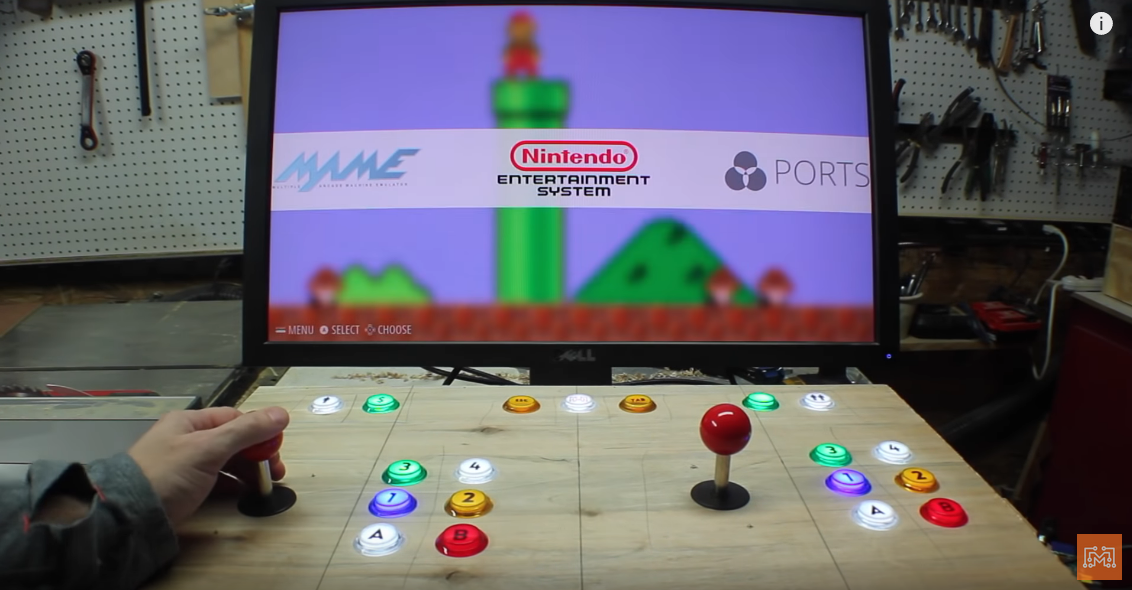
\includegraphics[width=.6\textwidth]{img/retropie.png}
\caption{Consola retropie realizada por ``I Like To Make Stuff''}
\label{fig:retropie}
\end{figure}


